\pdfminorversion=4
\documentclass[aspectratio=169]{beamer}

\mode<presentation>
{
  \usetheme{default}
  \usecolortheme{default}
  \usefonttheme{default}
  \setbeamertemplate{navigation symbols}{}
  \setbeamertemplate{caption}[numbered]
  \setbeamertemplate{footline}[frame number]  % or "page number"
  \setbeamercolor{frametitle}{fg=white}
  \setbeamercolor{footline}{fg=black}
} 

\usepackage[english]{babel}
\usepackage[utf8x]{inputenc}
\usepackage{tikz}
\usepackage{courier}
\usepackage{array}
\usepackage{bold-extra}
\usepackage{minted}
\usepackage[thicklines]{cancel}
\usepackage{fancyvrb}

\xdefinecolor{dianablue}{rgb}{0.18,0.24,0.31}
\xdefinecolor{darkblue}{rgb}{0.1,0.1,0.7}
\xdefinecolor{darkgreen}{rgb}{0,0.5,0}
\xdefinecolor{darkgrey}{rgb}{0.35,0.35,0.35}
\xdefinecolor{darkorange}{rgb}{0.8,0.5,0}
\xdefinecolor{darkred}{rgb}{0.7,0,0}
\definecolor{darkgreen}{rgb}{0,0.6,0}
\definecolor{mauve}{rgb}{0.58,0,0.82}

\title[2019-05-22-colloquium-languages]{Programming languages and particle physics}
\author{Jim Pivarski}
\institute{Princeton University -- IRIS-HEP}
\date{May 8, 2019}

%% Title: Programming languages and particle physics

%% Abstract:

%% Programming languages aren't for computers; they're for people. If a language doesn't make it easier to express your physics problem, it's not a suitable language. Some fields have specialized "Domain Specific Languages" (DSLs) that trade freedom of expression for focus on the problem at hand, and can even improve performance by limiting this scope. A prime example is SQL, widely used by data analysts outside of physics, which trades generic computation for a SELECT-WHERE-GROUPBY pattern. Interestingly, this was the design pattern of the first electromechanical computers (Hollerith machine, 1890) and it's still a major focus of big data today (Dean & Ghemawat: MapReduce, 2004). Particle physics problems don't fit SQL well; in fact, physicists became involved in computing in tandem with the invention of generic, digital computers (Von Neumann's stored-program machine, 1945). I will present some history, some general features of programming languages, what "declarative" really means, and will show some perhaps surprising examples of DSLs you're already using.

\usetikzlibrary{shapes.callouts}

\begin{document}

\logo{\pgfputat{\pgfxy(0.11, 7.4)}{\pgfbox[right,base]{\tikz{\filldraw[fill=dianablue, draw=none] (0 cm, 0 cm) rectangle (50 cm, 1 cm);}\mbox{\hspace{-8 cm}
\includegraphics[height=1 cm]{princeton-logo-long.png}\hspace{0.1 cm}\raisebox{0.1 cm}{
\includegraphics[height=0.8 cm]{iris-hep-logo-long.png}}\hspace{0.1 cm}}}}}

\begin{frame}
  \titlepage
\end{frame}

\logo{\pgfputat{\pgfxy(0.11, 7.4)}{\pgfbox[right,base]{\tikz{\filldraw[fill=dianablue, draw=none] (0 cm, 0 cm) rectangle (50 cm, 1 cm);}\mbox{\hspace{-8 cm}
\includegraphics[height=1 cm]{princeton-logo.png}\hspace{0.1 cm}\raisebox{0.1 cm}{
\includegraphics[height=0.8 cm]{iris-hep-logo.png}}\hspace{0.1 cm}}}}}

% Uncomment these lines for an automatically generated outline.
%\begin{frame}{Outline}
%  \tableofcontents
%\end{frame}

% START START START START START START START START START START START START START

\begin{frame}{}
\vspace{-0.1 cm}
\begin{columns}
\column{1.15\linewidth}
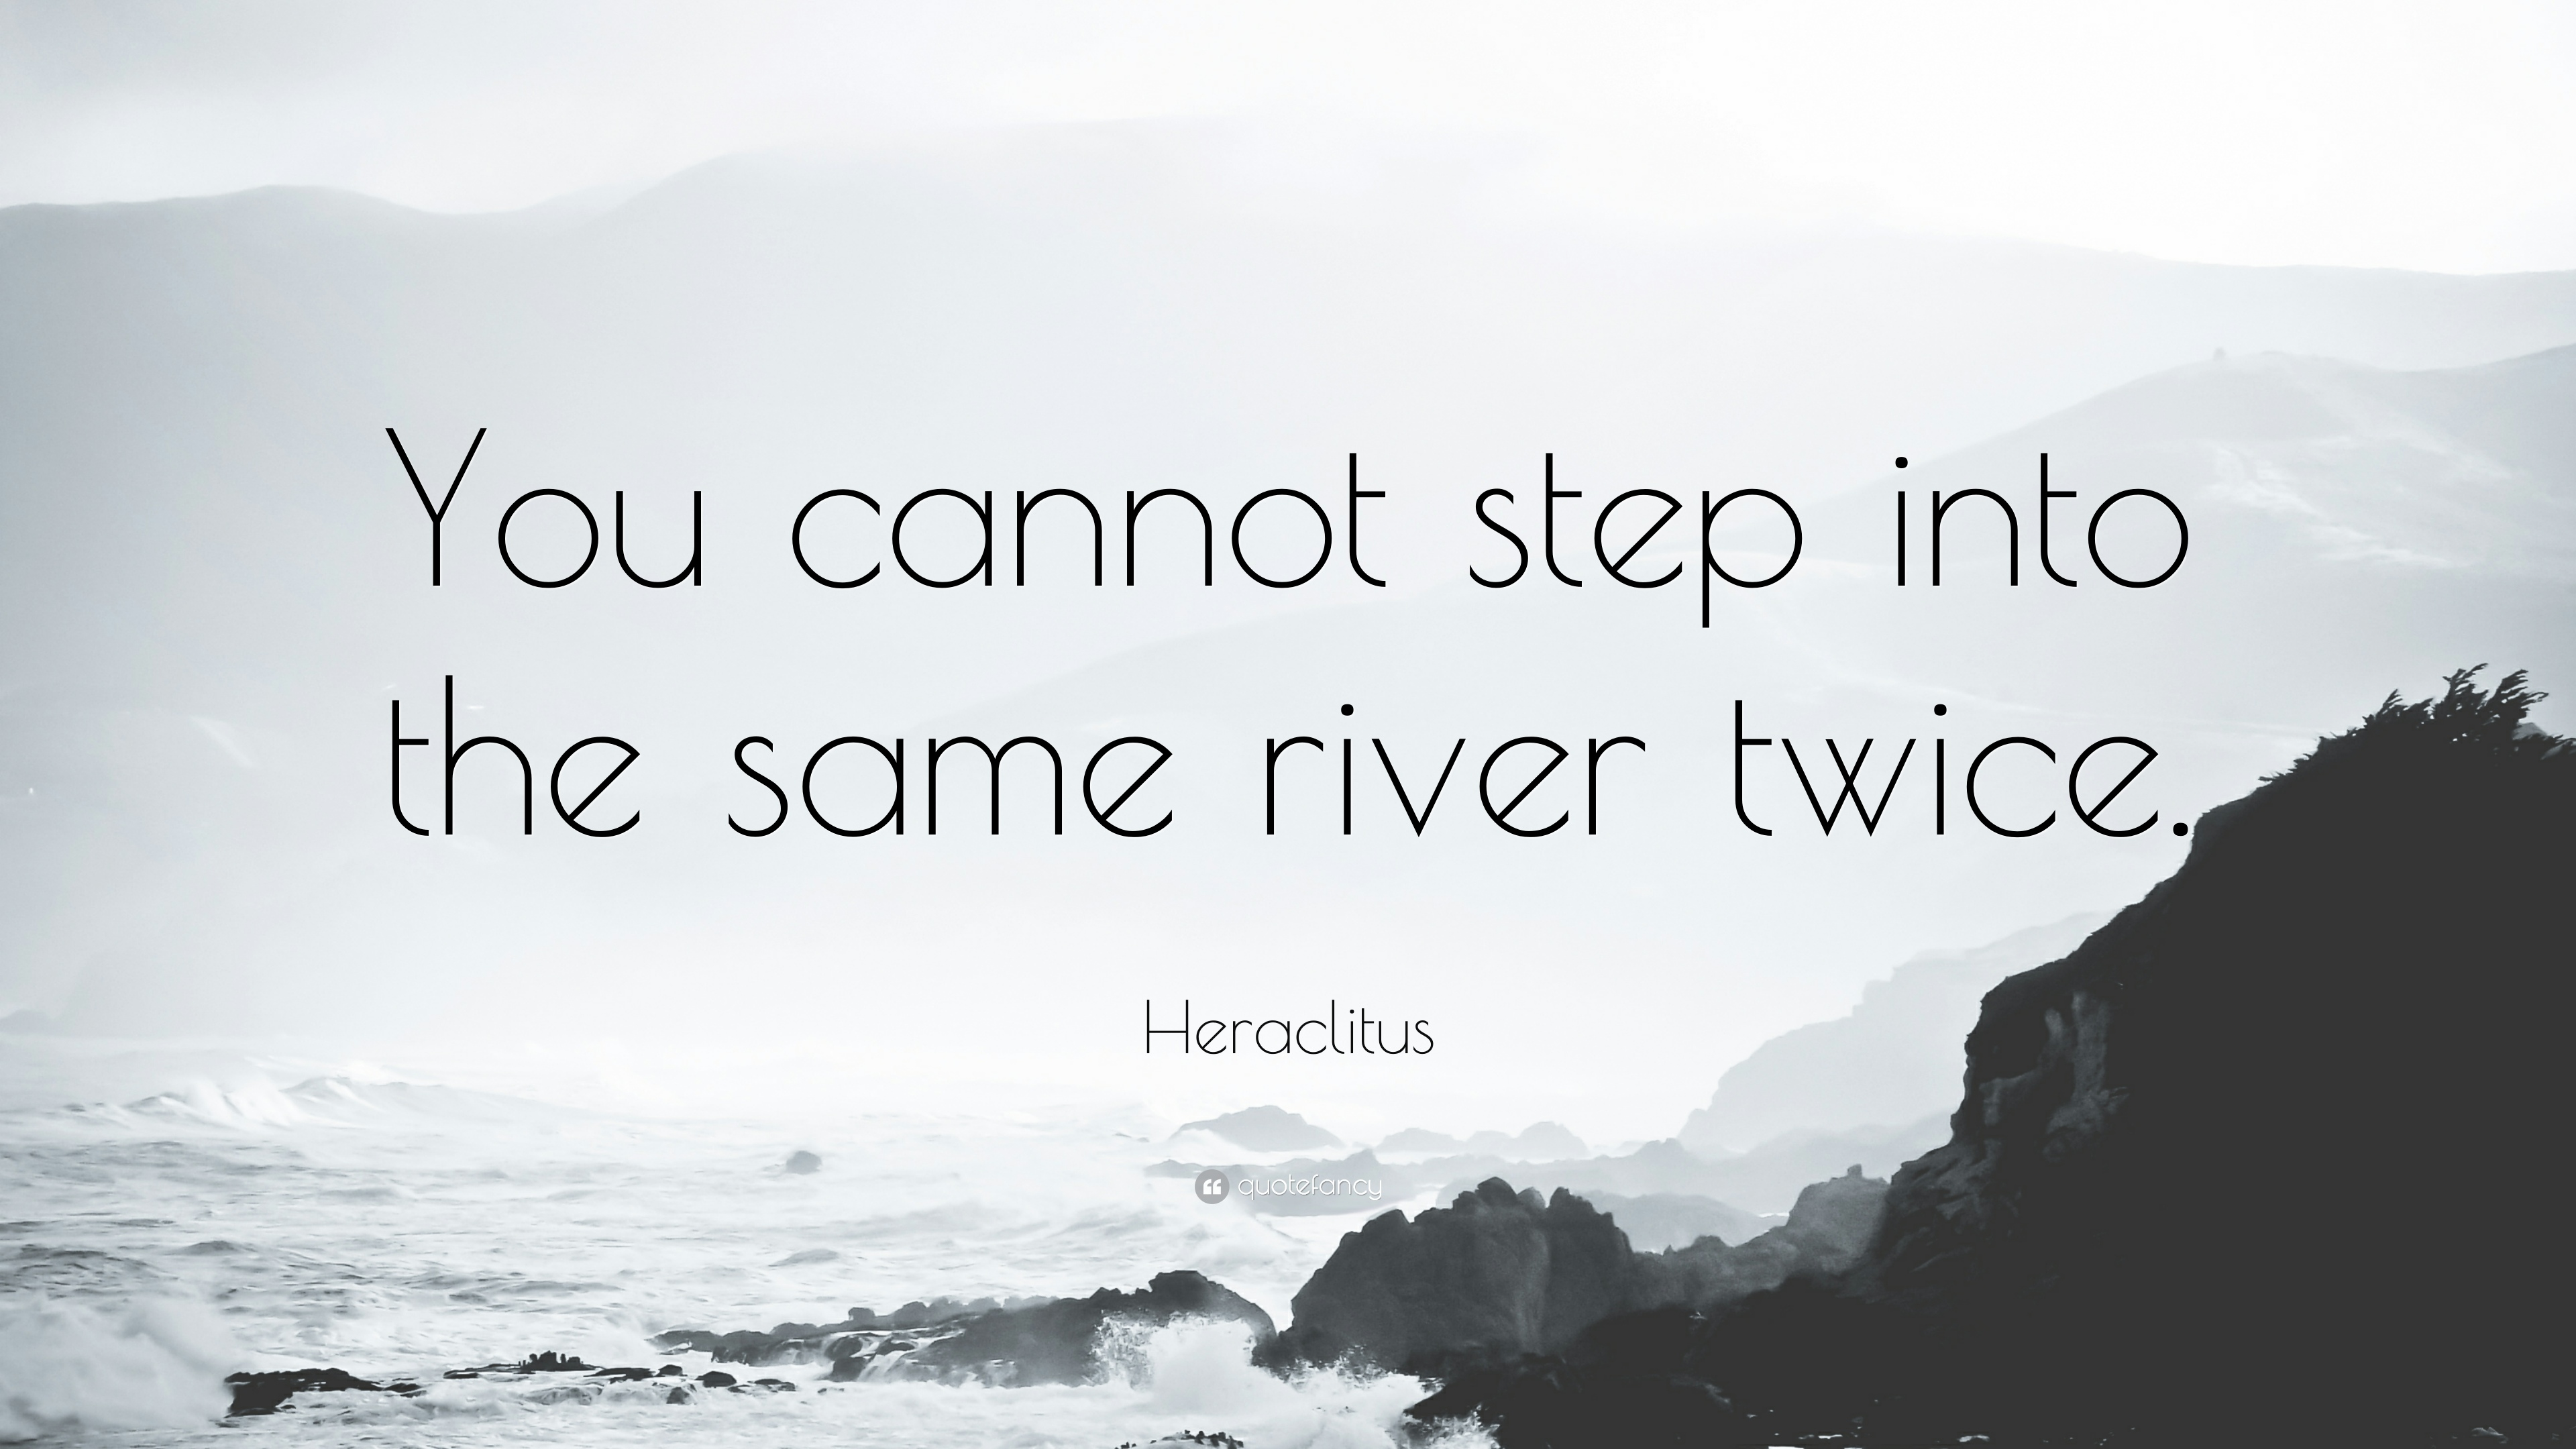
\includegraphics[width=\linewidth]{same-river-twice.jpg}
\end{columns}
\end{frame}

\begin{frame}{}
\huge
\vspace{0.5 cm}
\begin{center}
Because, you know, it's different water.
\end{center}
\end{frame}

\begin{frame}{}
\Large
\vspace{1.5 cm}
\begin{columns}
\column{1.02\linewidth}
\textcolor{darkblue}{\huge Why do we say it's the same river?}

\vspace{0.5 cm}
\uncover<2->{We associate an enormous number of microscopic states (``molecules here, molecules there'') with a single macroscopic state (``the river'').}
\end{columns}

\vspace{0.5 cm}
\begin{uncoverenv}<3->
\begin{columns}
\column{0.3\linewidth}
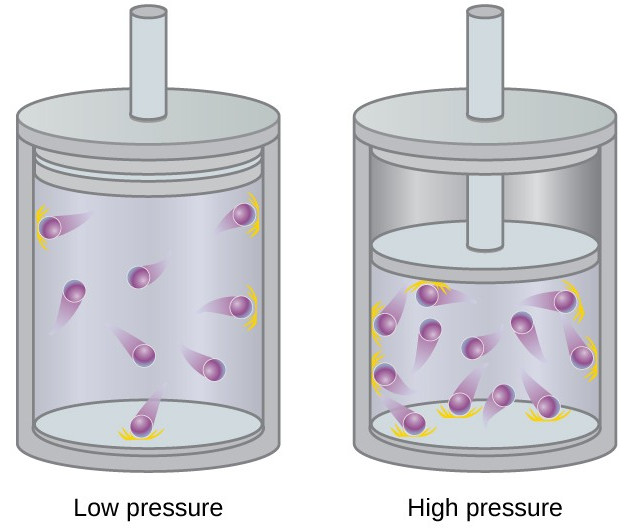
\includegraphics[width=\linewidth]{idealgas.jpg}

\column{0.6\linewidth}
This abstraction is thermodynamics, and it can be exact with the right definitions.
\end{columns}
\end{uncoverenv}
\end{frame}

\begin{frame}[fragile]{Much of computer science is about abstracting details, too.}
\scriptsize
\vspace{0.05 cm}
\begin{minted}{c++}
double bessel_j0(double x) {
    double out;
    if (fabs(x) < 8.0) {
        double y = x*x;
        double ans1 = 57568490574.0 + y*(-13362590354.0 + y*(651619640.7
                      + y*(-11214424.18 + y*(77392.33017 + y*(-184.9052456)))));
        double ans2 = 57568490411.0 + y*(1029532985.0 + y*(9494680.718
                      + y*(59272.64853 + y*(267.8532712 + y*1.0))));
        out = ans1 / ans2;
    }
    else {
        double z = 8.0 / fabs(x);
        double y = z*z;
        double xx = fabs(x) - 0.785398164;
        double ans1 = 1.0 + y*(-0.1098628627e-2 + y*(0.2734510407e-4
                      + y*(-0.2073370639e-5 + y*0.2093887211e-6)));
        double ans2 = -0.1562499995e-1 + y*(0.1430488765e-3
                      + y*(-0.6911147651e-5 + y*(0.7621095161e-6
                      - y*0.934935152e-7)));
        out = sqrt(0.636619772/fabs(x))*(cos(xx)*ans1 - z*sin(xx)*ans2);
    }
    return out;
}
\end{minted}

\vspace{-7.95 cm}\hspace{6 cm}{\uncover<2->{\LARGE $\leftarrow$ one value goes in}}

\vspace{6.4 cm}\hspace{6 cm}{\uncover<3->{\LARGE $\leftarrow$ one value comes out}}

\end{frame}

\begin{frame}{}
\Large
\vspace{0.97 cm}
\begin{columns}
\column{0.5\linewidth}
\mbox{\hspace{-3.5 cm}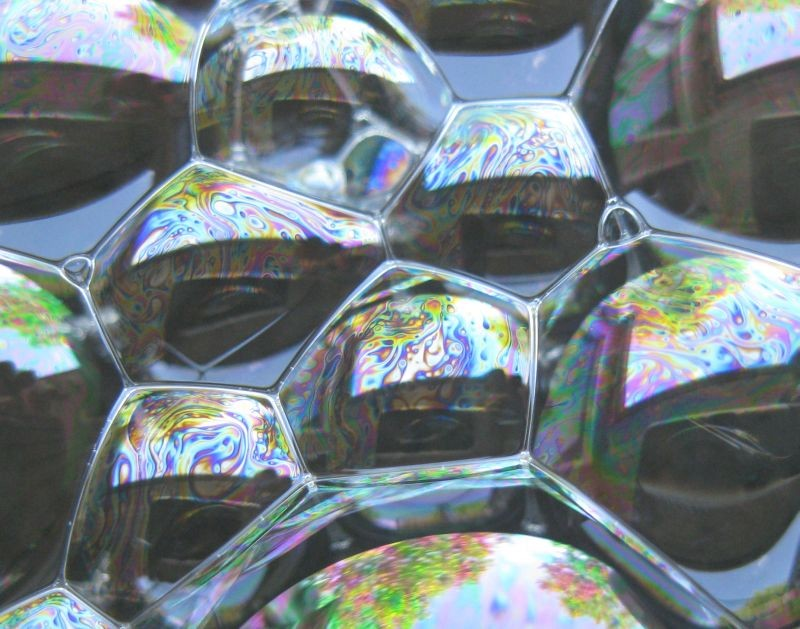
\includegraphics[height=8 cm]{soap-bubbles.jpg}}

\column{0.55\linewidth}
\textcolor{darkblue}{The abstraction is cumulative:}

\vspace{0.25 cm}
Every function/class/module has an interior and an interface---minimizing

\[ \frac{\mbox{\#external parameters}}{\mbox{\#internal parameters}} \]

\vspace{0.25 cm}
reduces the mental burden on programmers and users.
\end{columns}
\end{frame}

\begin{frame}{Science has layers of abstraction}
\large
\vspace{0.75 cm}
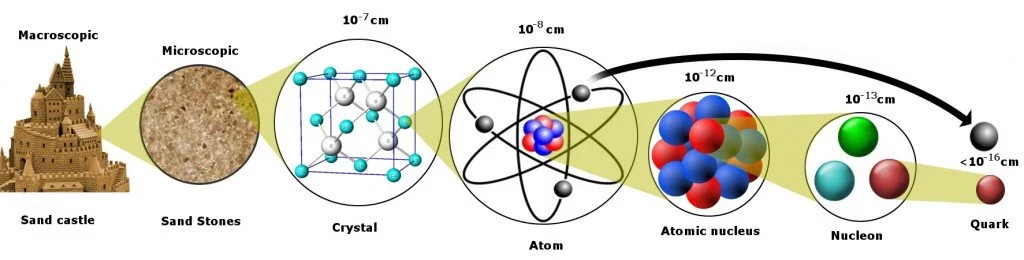
\includegraphics[width=\linewidth]{atom-proton-quark.png}

\vspace{1 cm}
\textcolor{gray}{though these are approximate, taking advantage of a separation of scales.}
\end{frame}

\begin{frame}{(cartoon diagram, not to scale)}
\vspace{0.2 cm}
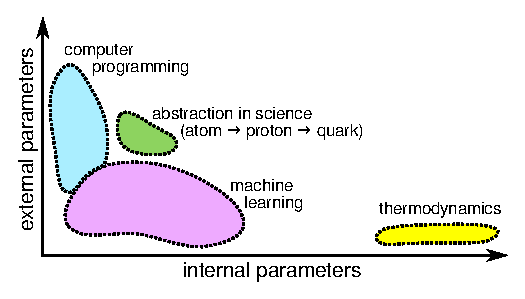
\includegraphics[width=\linewidth]{internal-vs-external.pdf}
\end{frame}

\begin{frame}{Software interfaces can be exact, despite radical internal differences.}
\large
\vspace{0.13 cm}
\begin{itemize}
\item Super Mario Bros.\ entirely rewritten in Javascript by Josh Goldberg.
\item Shares none of the original code: \textcolor{darkblue}{is it the same program?}
\end{itemize}

\begin{center}
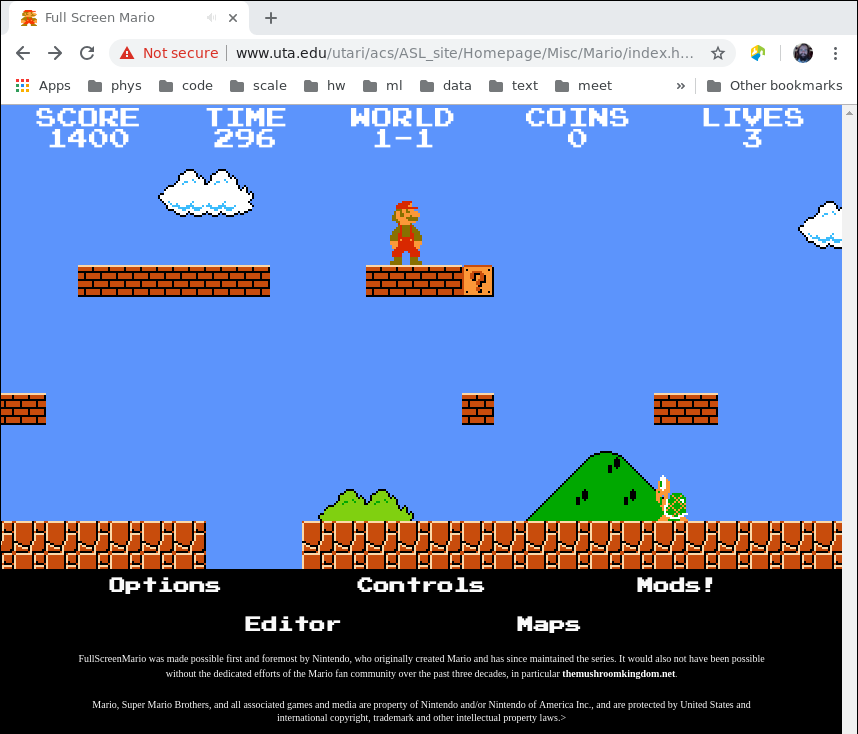
\includegraphics[width=0.97\linewidth]{supermario-javascript.png}
\end{center}
\end{frame}

\begin{frame}{}
\vspace{1.25 cm}
\Large
\begin{columns}
\column{0.65\linewidth}
\begin{center}
As a young programmer, I wasn't satisfied with high-level languages because I wanted to get down to the ``real'' computer.

\vspace{0.75 cm}
\uncover<2->{Which meant Pascal. \\ Pascal was ``real,'' and BASIC was not.}

\vspace{0.75 cm}
\uncover<3->{But ultimately, not even machine code is real in the sense that I meant.}
\end{center}
\column{0.35\linewidth}
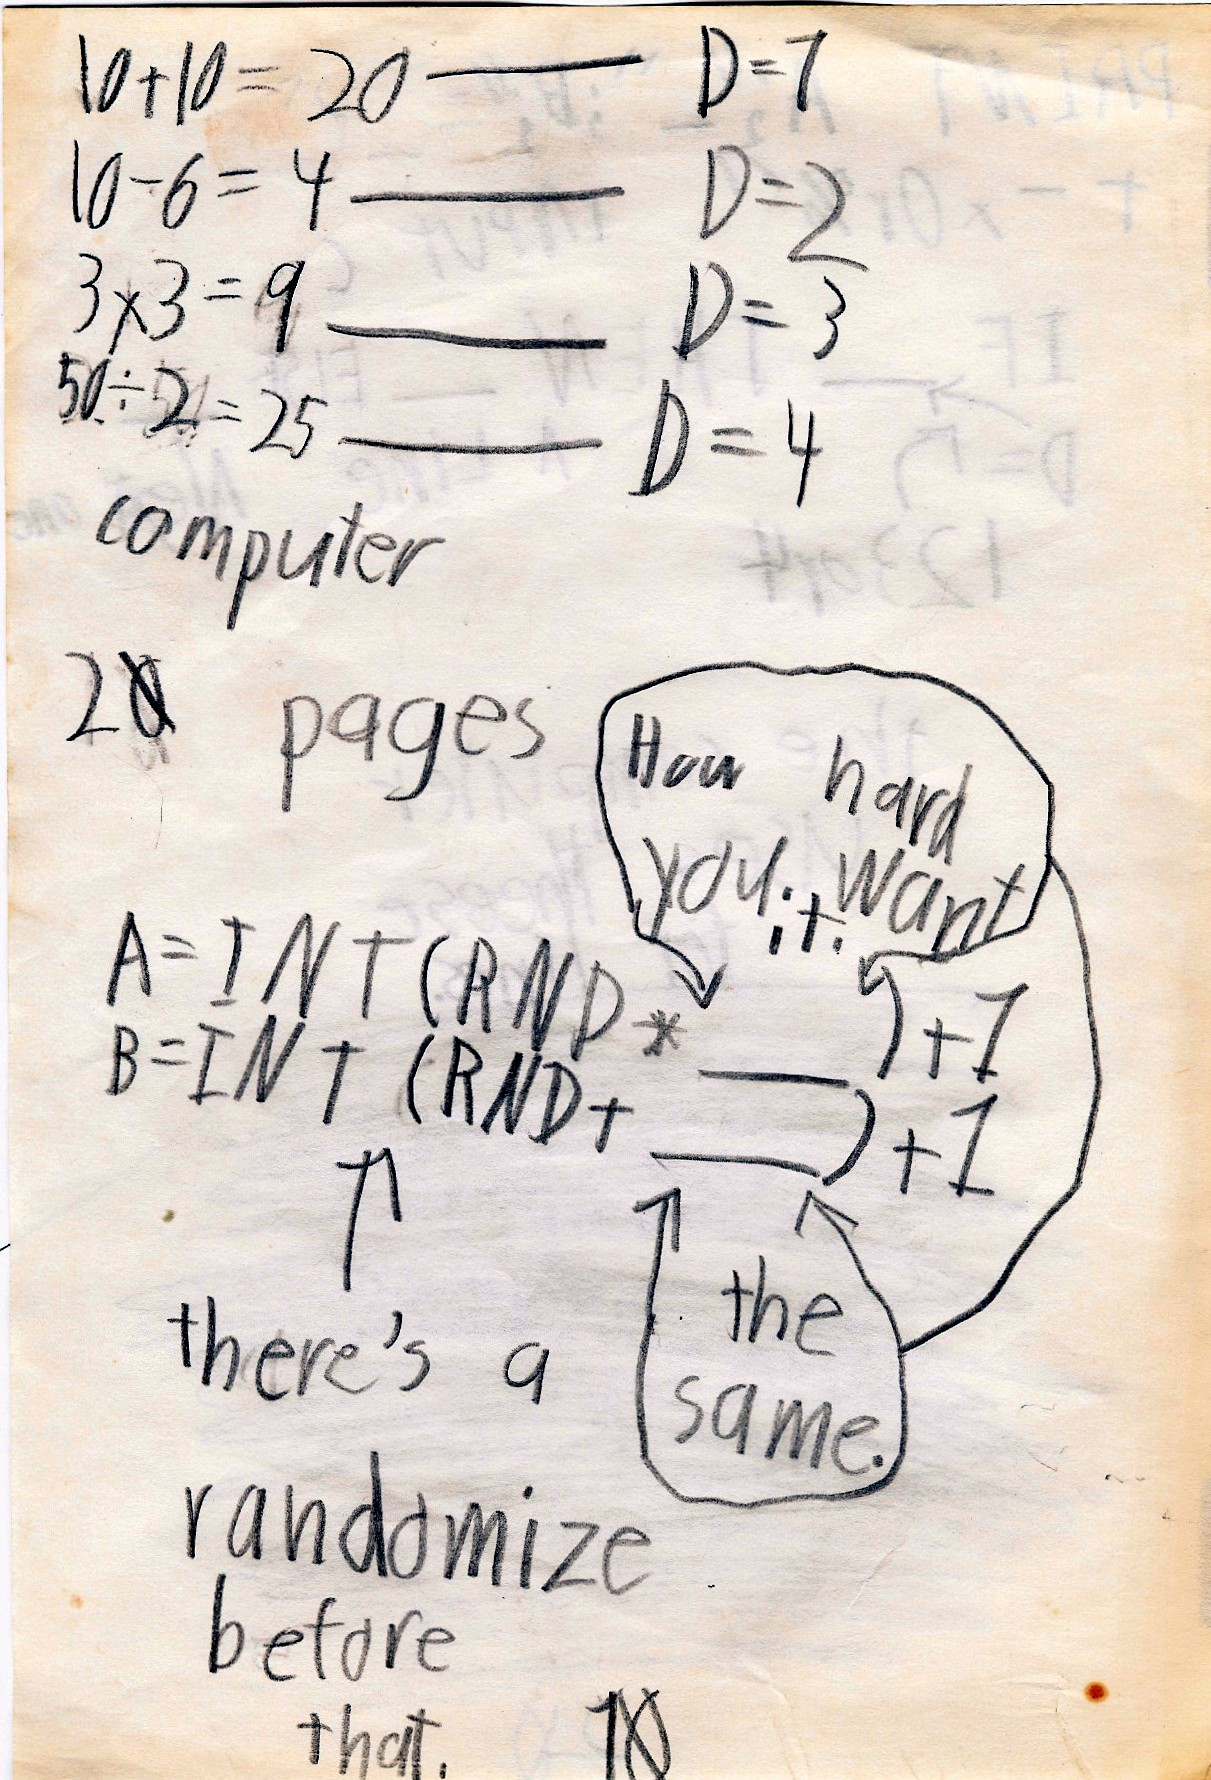
\includegraphics[width=\linewidth]{jimbasic1.jpg}
\end{columns}
\end{frame}

\begin{frame}{}
\LARGE
\vspace{1 cm}
\begin{center}
A computer is a set of physical states \\ {\it that we interpret} as computations.

\vspace{0.2 cm}
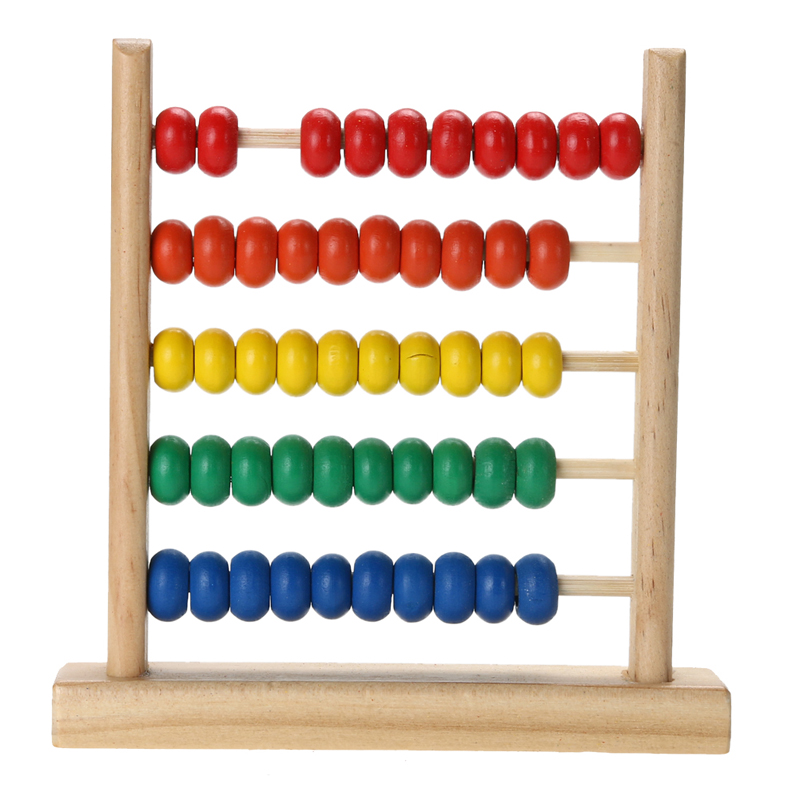
\includegraphics[width=0.4\linewidth]{abacus.jpg}
\end{center}
\end{frame}

\begin{frame}{Programming languages are how we describe those computations.}
\Large
\vspace{0.1 cm}
\begin{center}
Some languages are better than others.
\end{center}

\vspace{0.1 cm}
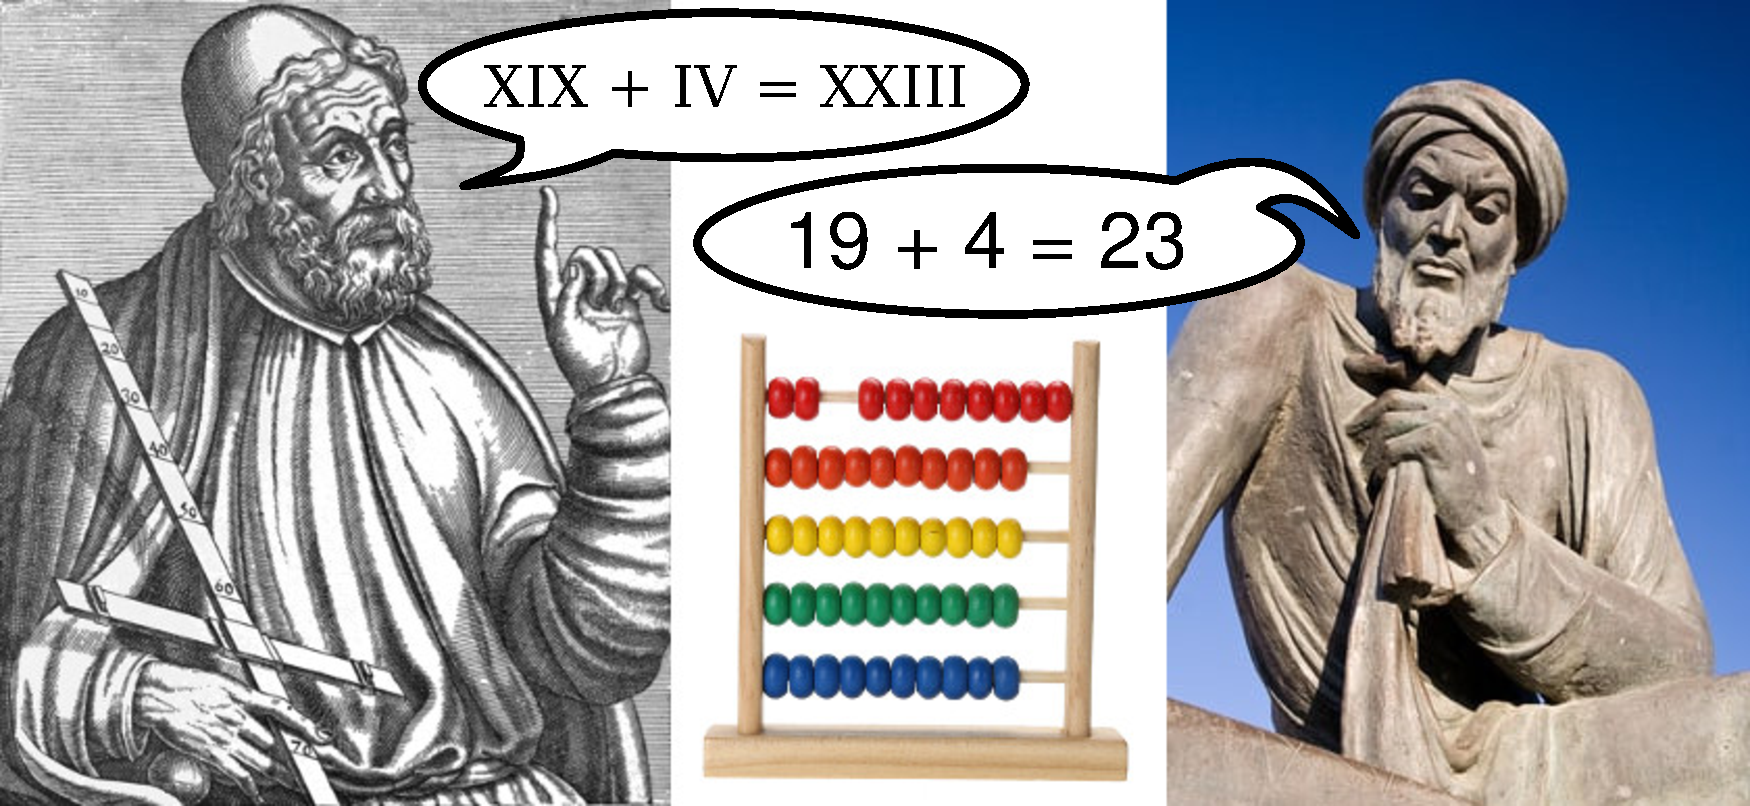
\includegraphics[width=\linewidth]{abacus_ptolemy_al-khwarizmi.pdf}
\end{frame}

\begin{frame}{}
\Large
\vspace{1.25 cm}
\begin{center}
Some programming languages are high-level and others low-level, \\
but {\it all} programming languages are for humans, not computers.

\vspace{0.75 cm}
\begin{uncoverenv}<2->
Each one re-expresses the programmer's intent in terms of another:

\large
\vspace{0.25 cm}
\begin{tabular}{r c l}
CMSSW configuration & \textcolor{darkblue}{implemented in} & Python runtime \\
Python runtime & \textcolor{darkblue}{implemented in} & C source code \\
C source code & \textcolor{darkblue}{compiled into} & machine instructions \\
machine instructions & \textcolor{darkblue}{built into} & logic gates \\
logic gates & \textcolor{darkblue}{interpreted as} & computation
\end{tabular}

\vspace{0.25 cm}
\Large and the last level is a human interpretation.
\end{uncoverenv}
\end{center}
\end{frame}


%% \begin{frame}[fragile]
%% \frametitle{Map-reduce}

%% Hadoop executes two sets of independent, identical processors:
%% \begin{itemize}
%% \item Mappers, which transform each input to a $\langle$key, value$\rangle$ pair.
%% \item Reducers, each operates on all values that have a given key.
%% \end{itemize}

%% \vspace{-0.1 cm}
%% \begin{columns}
%% \column{0.5\linewidth}
%% \begin{lstlisting}[frame=single]
%% def mapper($webpage$):
%%   for $word$ in $webpage$.split():
%%     yield ($word$, $webpage$)
%% $$
%% \end{lstlisting}
%% \column{0.58\linewidth}
%% \begin{lstlisting}[frame=single]
%% def reducer($word$, $webpages$):
%%   searchIndex[$word$] = {}
%%   for $webpage$ in $webpages$:
%%     searchIndex[$word$].add($webpage$)
%% \end{lstlisting}
%% \end{columns}

%% The system groups data by key in an optimized way (independent partial sorts followed by merge, minimizing network bandwidth).

%% \vspace{0.2 cm}
%% \mbox{ } \hfill 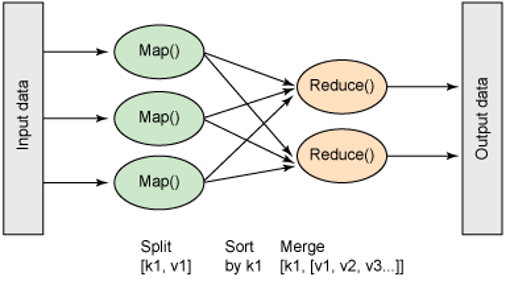
\includegraphics[width=0.6\linewidth]{PLOTS/mapreduce-diagram-by-ibm.png} \hfill \mbox{ }
%% \end{frame}

%% \begin{frame}[fragile]{Nested query in C++}
%% \vspace{0.5 cm}
%% {\bf Example query:}
%% \begin{center}
%% \begin{minipage}{0.95\linewidth}
%% \textcolor{darkblue}{``Momentum of the track with $|\eta|$ $<$ 2.4 that has the most hits.''}
%% \end{minipage}
%% \end{center}
%% \small
%% \begin{minted}{c++}
%% Track *best = NULL;
%% for (int i = 0;  i < tracks.size();  i++) {
%%   if (fabs(tracks[i]->eta) < 2.4)
%%     if (best == NULL ||
%%         tracks[i]->hits.size() > best->hits.size())
%%       best = tracks[i];
%% }
%% if (best != NULL)
%%   return best->pt;
%% else
%%   return 0.0;
%% \end{minted}
%% \end{frame}

%% \begin{frame}[fragile]{Nested query in SQL}
%% \vspace{0.5 cm}
%% {\bf Example query:}
%% \begin{center}
%% \begin{minipage}{0.95\linewidth}
%% \textcolor{darkblue}{``Momentum of the track with $|\eta|$ $<$ 2.4 that has the most hits.''}
%% \end{minipage}
%% \end{center}
%% \small
%% \begin{minted}{sql}
%% WITH hit_stats AS (
%%   SELECT hit.track_id, COUNT(*) AS hit_count FROM hit
%%     GROUP BY hit.track_id),
%%  track_sorted AS (
%%     SELECT track.*, 
%%     ROW_NUMBER() OVER (
%%      PARTITION BY track.event_id
%%      ORDER BY hit_stats.hit_count DESC)
%%   track_ordinal FROM track INNER JOIN hit_stats
%%     ON hit_stats.track_id = track.id
%%     WHERE ABS(track.eta) < 2.4)
%%  SELECT * FROM event INNER JOIN track_sorted
%%    ON track_sorted.event_id = event.id
%% WHERE
%%   track_sorted.track_ordinal = 1
%% \end{minted}
%% \end{frame}

%% \begin{frame}[fragile]{}
%% 50$\times$

%% \scriptsize
%% \begin{onlyenv}<1>
%% \begin{minted}{python}
%% import time
%% import numpy

%% def run_python(height, width, maxiterations=20):
%%     y, x = numpy.ogrid[-1:0:height*1j, -1.5:0:width*1j]
%%     c = x + y*1j
%%     fractal = numpy.full(c.shape, maxiterations, dtype=numpy.int32)
%%     for h in range(height):
%%         for w in range(width):                  # for each pixel (h, w)...
%%             z = c[h, w]
%%             for i in range(maxiterations):      # iterate at most 20 times
%%                 z = z**2 + c[h, w]              # applying z → z² + c
%%                 if abs(z) > 2:                  # if it diverges (|z| > 2)
%%                     fractal[h, w] = i           # color the plane with the iteration number
%%                     break                       # we're done, no need to keep iterating
%%     return fractal
%% \end{minted}
%% \end{onlyenv}
%% \begin{onlyenv}<2>
%% \begin{minted}{python}
%% import numba

%% @numba.jit
%% def run_numba(height, width, maxiterations=20):
%%     y, x = numpy.ogrid[-1:0:height*1j, -1.5:0:width*1j]
%%     c = x + y*1j
%%     fractal = numpy.full(c.shape, maxiterations, dtype=numpy.int32)
%%     for h in range(height):
%%         for w in range(width):                  # for each pixel (h, w)...
%%             z = c[h, w]
%%             for i in range(maxiterations):      # iterate at most 20 times
%%                 z = z**2 + c[h, w]              # applying z → z² + c
%%                 if abs(z) > 2:                  # if it diverges (|z| > 2)
%%                     fractal[h, w] = i           # color the plane with the iteration number
%%                     break                       # we're done, no need to keep iterating
%%     return fractal
%% \end{minted}
%% \end{onlyenv}

%% \end{frame}

\end{document}
